\section{Camera Geometry}
The camera is a projection device mapping 3D world points to 2D image pixels. The location of the pixel in the image plane has a direct relationship with the location of the point in the 3D world.
Approximating the camera with a pinhole model loses depth information. 

Since camera positioning dictates scene perception, this section outlines core camera geometry principles.

\subsection{Affine Transformations}
An affine transformation is a spatial operation represented by multiplying a \textbf{homogeneous point} by a transformation matrix. 
Key transformations include \textbf{scaling}, \textbf{rotation}, \textbf{translation}, and their \textbf{composition}. 
These serve as the foundational building blocks for 2D and 3D camera matrices.

\subsubsection{Homogeneous Coordinates}
A 2D pixel is standardly represented as $p = \begin{bmatrix} x, y \end{bmatrix}^T$. 
Using homogeneous coordinates allows us to easily compute projective transformations and represent points at infinity by appending a scaling factor $s$ (typically $s=1$):
\[ p = \begin{bmatrix} sx, sy, s \end{bmatrix}^T \]

Similarly, a standard 3D point $P = \begin{bmatrix} X, Y, Z \end{bmatrix}^T$ is represented in homogeneous coordinates as:
\[ P = \begin{bmatrix} sX, sY, sZ, s \end{bmatrix}^T \]

\subsubsection{Scaling}
Scaling resizes an object by multiplying point coordinates by scaling factors. The transformation is uniform if all factors are equal.

\paragraph{2D Case} The scaled coordinates $(x', y')$ are computed using the scaling matrix $S_{c_x, c_y}$:
\[ \begin{bmatrix} x' \\ y' \end{bmatrix} = \begin{bmatrix} c_x & 0 \\ 0 & c_y \end{bmatrix} \begin{bmatrix} x \\ y \end{bmatrix} \]

\paragraph{3D Case} Scaling extends to the z-coordinate via a 4x4 transformation matrix:
\[ ^2P_i = S(s_x, s_y, s_z) ^1P_i, \qquad S(s_x, s_y, s_z) = \begin{bmatrix}
s_x & 0 & 0 & 0 \\
0 & s_y & 0 & 0 \\
0 & 0 & s_z & 0 \\
0 & 0 & 0 & 1
\end{bmatrix} \]

\subsubsection{Rotation}
Rotation changes an object's orientation around the origin.

\paragraph{2D Case} Rotation by angle $\theta$ (in radians) uses the matrix $R_{\theta}$:
\[ \begin{bmatrix} x' \\ y' \end{bmatrix} = \begin{bmatrix} \cos \theta & -\sin \theta \\ \sin \theta & \cos \theta \end{bmatrix} \begin{bmatrix} x \\ y \end{bmatrix} \]

\paragraph{3D Case} Rotations around the x, y, and z axes require specific 4x4 matrices:
\begin{itemize}
\item \textbf{X-axis} ($\theta_x$):
\[ R(X, \theta_x) = \begin{bmatrix}
1 & 0 & 0 & 0 \\
0 & \cos \theta_x & -\sin \theta_x & 0 \\
0 & \sin \theta_x & \cos \theta_x & 0 \\
0 & 0 & 0 & 1
\end{bmatrix} \]
\item \textbf{Y-axis} ($\theta_y$):
\[ R(Y, \theta_y) = \begin{bmatrix}
\cos \theta_y & 0 & \sin \theta_y & 0 \\
0 & 1 & 0 & 0 \\
-\sin \theta_y & 0 & \cos \theta_y & 0 \\
0 & 0 & 0 & 1
\end{bmatrix} \]
\item \textbf{Z-axis} ($\theta_z$):
\[ R(Z, \theta_z) = \begin{bmatrix}
\cos \theta_z & -\sin \theta_z & 0 & 0 \\
\sin \theta_z & \cos \theta_z & 0 & 0 \\
0 & 0 & 1 & 0 \\
0 & 0 & 0 & 1
\end{bmatrix} \]
\end{itemize}

\subsubsection{Translation}
Translation shifts an object without altering shape or orientation, equivalent to moving the coordinate origin.

\paragraph{2D Case} To shift a point by $(x_0, y_0)$, we use a 3x3 matrix applied to homogeneous coordinates:
\[ \begin{bmatrix} x' \\ y' \\ 1 \end{bmatrix} = \begin{bmatrix} 1 & 0 & x_0 \\ 0 & 1 & y_0 \\ 0 & 0 & 1 \end{bmatrix} \begin{bmatrix} x \\ y \\ 1 \end{bmatrix} \]

\paragraph{3D Case} A 3D translation by $(t_x, t_y, t_z)$ uses a 4x4 matrix:
\[ T(t_x, t_y, t_z) = \begin{bmatrix}
1 & 0 & 0 & t_x \\
0 & 1 & 0 & t_y \\
0 & 0 & 1 & t_z \\
0 & 0 & 0 & 1
\end{bmatrix} \]

\subsection{2D Camera Matrix}
These transformations can be combined into a single \textbf{camera matrix}, which compactly maps real-world points to the 2D image plane.
The 2D camera matrix typically combines rotation, translation, and scaling.

\begin{figure}[H]
    \centering
    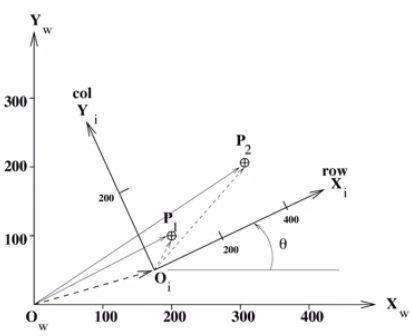
\includegraphics[width=0.5\textwidth]{../media/geometry/2D-camera_matrix.png}
    \caption{Camera matrix in the 2D case.}
\end{figure}
As seen in the figure, a real-world point $P_1$ is projected onto the image plane as $P_2$ by sequentially applying translation, 
rotation ($\theta$), and scaling ($s$).

In general, given a real-world point $P_w$, its transformation to the image plane $P_i$ is expressed as:
$$P_i = S_{s_x, s_y} R_{\theta} D_{x_0, y_0} P_w$$
where $D_{x_0, y_0}$ is the translation matrix, $R_{\theta}$ is the rotation matrix, and $S_{s_x, s_y}$ is the scaling matrix.

\paragraph{Computing the Camera Matrix}
To map a point from the real world to the image plane, we theoretically multiply the individual scaling, rotation, and translation matrices:
\[
    \begin{bmatrix} x_i \\ y_i \\ 1 \end{bmatrix} = 
    \underbrace{ 
        \begin{bmatrix} c_x & 0 & 0 \\ 0 & c_y & 0 \\ 0 & 0 & 1 \end{bmatrix} 
        \begin{bmatrix} \cos \theta & -\sin \theta & 0 \\ \sin \theta & \cos \theta & 0 \\ 0 & 0 & 1 \end{bmatrix} 
        \begin{bmatrix} 1 & 0 & x_0 \\ 0 & 1 & y_0 \\ 0 & 0 & 1 \end{bmatrix} 
    }_{\text{Complex non-linear system}}
    \begin{bmatrix} x_w \\ y_w \\ 1 \end{bmatrix} 
\]

However, solving directly for these physical parameters ($\theta, c_x, c_y, x_0, y_0$) is mathematically difficult due to the trigonometric functions and multiplied variables. 

To simplify the math, we multiply these three $3 \times 3$ matrices together and abstract the resulting cells into generic coefficients. This creates a \textbf{single, general camera matrix} $C$:
$$C = \begin{bmatrix} a_{11} & a_{12} & a_{13} \\ a_{21} & a_{22} & a_{23} \\ 0 & 0 & 1 \end{bmatrix}$$

This transforms our complex problem into a simple linear mapping equation:
$$P_i = C P_w$$

Because this generalized matrix $C$ has 6 unknown parameters ($a_{11}$ through $a_{23}$), we need at least 3 \textbf{control points} to estimate it. Control points are reference points with known coordinates that are clearly identifiable in both the real world and the image plane. Each control point provides 2 equations (one for the x-coordinate, one for the y-coordinate).

\note{Control point selection guidelines:
    \begin{itemize}
        \item \textbf{Visibility:} Must be clearly identifiable in both spaces to ensure accurate matching.
        \item \textbf{Distribution:} Should be widely spread. Avoid collinear or highly clustered points to prevent numerical instability.
        \item \textbf{Quantity:} While 3 points are mathematically sufficient to find the 6 parameters, using more provides a robust estimation against noise using the Least Squares approach.
    \end{itemize}
}

\paragraph{Least Squares Approach}
When using more control points than the minimum required, the goal is to find the parameters that minimize the squared \textbf{error}
between the projected points and the actual points in the image plane.

For $N$ points, where a real-world point $(x_j, y_j)$ maps to an actual image point $(u_j, v_j)$, the error $E$ is:
$$E = \sum_{j=1}^{N} \left( \underbrace{\left(a_{11} x_j + a_{12} y_j + a_{13}\right)}_{\text{projected } u_j} - u_j \right)^2 + \left( \underbrace{\left(a_{21} x_j + a_{22} y_j + a_{23}\right)}_{\text{projected } v_j} - v_j \right)^2$$

This optimization problem is solved by computing the partial derivatives of the error function with respect to the 6 matrix parameters and setting them to zero. This yields the following linear system:
$$\begin{bmatrix} 
\sum x_j^2 & \sum x_j y_j & \sum x_j & 0 & 0 & 0 \\ 
\sum x_j y_j & \sum y_j^2 & \sum y_j & 0 & 0 & 0 \\ 
\sum x_j & \sum y_j & N & 0 & 0 & 0 \\ 
0 & 0 & 0 & \sum x_j^2 & \sum x_j y_j & \sum x_j \\ 
0 & 0 & 0 & \sum x_j y_j & \sum y_j^2 & \sum y_j \\ 
0 & 0 & 0 & \sum x_j & \sum y_j & N 
\end{bmatrix} 
\begin{bmatrix} a_{11} \\ a_{12} \\ a_{13} \\ a_{21} \\ a_{22} \\ a_{23} \end{bmatrix} = 
\begin{bmatrix} \sum x_j u_j \\ \sum y_j u_j \\ \sum u_j \\ \sum x_j v_j \\ \sum y_j v_j \\ \sum v_j \end{bmatrix}$$

This system can be solved using standard linear algebra techniques, such as Gaussian elimination or Singular Value Decomposition (SVD), to find the optimal parameters for the camera matrix $C$.

\subsection{3D Camera Matrix}
The 2D camera matrix assumes the camera faces a flat surface perfectly parallel to the image plane. 
For a real-world 3D scene, we must account for camera \textbf{calibration}, the process of estimating the camera's \textbf{intrinsic} and \textbf{extrinsic} parameters.

\subsubsection{Calibration Parameters}
\begin{itemize}
    \item \textbf{Intrinsic:} Internal, sensor-specific characteristics (e.g., focal length, pixel size, image distortion). 
    These dictate how 3D rays project onto the 2D sensor and are specific to each sensor.
    \item \textbf{Extrinsic:} The position (translation) and orientation (rotation) of the camera in the 
    3D world relative to a reference coordinate system.
\end{itemize}

\paragraph{Coordinate Systems}
A 3D point can be represented in several frames of reference:
\begin{itemize}
    \item \textbf{Model/World Coordinate System:} The real-world origin and axes (often tied to a specific 3D model in the scene).
    \item \textbf{Camera Coordinate System:} Defined in 3D space with its origin at the camera's optical center and axes aligned with the camera's orientation.
    \item \textbf{Image Coordinate System:} The 2D pixel grid of the camera sensor, where the origin is typically at the top-left corner.
\end{itemize}

\note{Notation: We denote a pixel $P_i$ in the coordinate system of camera $k$ as $^kP_i$.}

\subsubsection{General Transformation Matrix}
We can combine 3D rotations and translations into a single $4 \times 4$ General Transformation Matrix $C$. This maps points between different 3D camera coordinate systems (e.g., from Camera 1 to Camera 2: $^2P_i = C ^1P_i$):
$$ C = \begin{bmatrix}
r_{11} & r_{12} & r_{13} & t_x \\
r_{21} & r_{22} & r_{23} & t_y \\
r_{31} & r_{32} & r_{33} & t_z \\
0 & 0 & 0 & 1
\end{bmatrix} $$

\subsubsection{The Full Camera Matrix}
The General Transformation Matrix only handles 3D-to-3D movements. To map a 3D world point $^WP$ to a 2D image pixel $^IP$, we need a complete \textbf{Camera Matrix} ($^I_WC$) that combines both extrinsic and intrinsic parameters:
$$ ^IP = ^I_WC ^WP $$

In homogeneous coordinates, this projection looks like:
$$ \begin{bmatrix}
s' P_x \\ s' P_y \\ s'
\end{bmatrix} =
^I_WC \begin{bmatrix}
^WP_x \\ ^WP_y \\ ^WP_z \\ 1
\end{bmatrix} $$

To build this final matrix, we apply three sequential transformations (mirroring a pinhole camera model):
\begin{enumerate}
    \item \textbf{Roto-Translation ($TR$):} Extrinsic mapping from the World coordinate system ($^WP$) to the 3D Camera coordinate system ($^CP$).
    \item \textbf{Projection ($\Pi$):} Intrinsic mapping from the 3D Camera system to an intermediate 2D image plane ($^FP$), measured in millimeters.
    \item \textbf{Pixel Scaling ($\mathcal{S}$):} Intrinsic conversion from physical millimeters ($^FP$) to discrete image pixels ($^IP$).
\end{enumerate}

Multiplying these steps together yields our final $3 \times 4$ Camera Matrix $C$:
$$ C = \begin{bmatrix}
c_{11} & c_{12} & c_{13} & c_{14} \\
c_{21} & c_{22} & c_{23} & c_{24} \\
c_{31} & c_{32} & c_{33} & 1 \\
\end{bmatrix} $$

\paragraph{Estimating the Matrix}
Because this matrix has 11 unknown parameters (12 entries minus the fixed scaling factor of 1), we need at least \textbf{6 control points} in the real world to solve for it. 
\begin{itemize}
    \item Calibration typically uses an object of known geometry (like a checkerboard) to extract these points.
    \item Since the estimation relies on specific control points, accuracy degrades for scene points that are far away or occluded. 
    \item As with the 2D case, we use extra control points and apply Least Squares optimization to minimize projection error.
\end{itemize}

\subsection{Binocular Stereo}
Binocular stereo is the simplest two-camera system for computing 3D world coordinates. 
It requires two cameras viewing the same scene from different perspectives; o
nly points visible to both cameras can be reconstructed.

To extract 3D information, the system performs two main steps:
\begin{itemize}
    \item \textbf{Correspondence Computing}: Matching the projections of the same 3D point across both image planes. 
    This uses feature matching and structural constraints—such as the \textbf{epipolar constraint} 
    (which states that corresponding points must lie on the same epipolar line, defined by the intersection of the image plane and the plane containing the camera centers and the 3D point) to significantly reduce the search space.
    \item \textbf{Reconstruction}: Triangulating the 3D world coordinates from the matched 2D projections. 
    This requires calibrated cameras (known intrinsic and extrinsic parameters). 
\end{itemize}

Due to occlusions and limited fields of view, a one-to-one mapping between the two cameras is never guaranteed. 
Unmatched points simply cannot be reconstructed in 3D.

\subsubsection{Reconstruction}
With known camera matrices, the 3D position of a point $[X, Y, Z]$ is computed by 
intersecting the rays projected from the matched 2D image points. Because projections are subject to noise and error, 
these two 3D rays rarely intersect perfectly. In practice, the estimated 3D position 
is chosen as the coordinate that minimizes the distance between the two non-intersecting rays.

\subsubsection{Co-Planar Cameras}
In a co-planar configuration, the two cameras and their image planes are perfectly parallel. 
This simplifies 3D coordinate computation because the only difference between the two projections is a horizontal shift along the x-axis. 
While this makes correspondence computing much easier, phenomena like parallax (where closer objects appear to move faster than distant ones) 
must be handled carefully when calculating the speed of moving objects.

\paragraph{Reconstruction for Co-Planar Cameras}
\begin{figure}[H]
    \centering
    \resizebox{\linewidth}{!}{\begin{tikzpicture}[
    scale=1.05,
    >=latex,
    point/.style={circle, fill, inner sep=1.8pt},
    projection/.style={circle, fill, inner sep=1.2pt},
    measure/.style={<->, thin},
    guide/.style={densely dashed, thin}
]

% ------------------------------------------------
% Coordinates
% ------------------------------------------------
\coordinate (Cl) at (0,0);      % left camera center
\coordinate (Cr) at (5,0);      % right camera center
\coordinate (WP) at (6.7,5.2);  % world point
\coordinate (Fl) at (0,1.15);   % left principal point
\coordinate (Fr) at (5,1.15);   % right principal point
\coordinate (WBase) at (6.7,0);
\coordinate (RMeasure) at (6.7,-1.35);

\path[name path=left ray] (Cl) -- (WP);
\path[name path=right ray] (Cr) -- (WP);
\path[name path=image plane] (-1.4,1.15) -- (8,1.15);
\path[name intersections={of=left ray and image plane, by=Pl}];
\path[name intersections={of=right ray and image plane, by=Pr}];

% ------------------------------------------------
% Axes
% ------------------------------------------------
\draw[->] (-1.35,0) -- (8,0) node[right] {$x$};
\draw[->] (0,-0.45) -- (0,6.25) node[above] {$z$};
\draw[thin] (-0.95,1.15) -- (1.85,1.15);
\draw[thin] (4.35,1.15) -- (7.15,1.15) node[right] {$z=f$};

% ------------------------------------------------
% Camera centers
% ------------------------------------------------
\node[point, label=below left:{$O_l=0$}] at (Cl) {};
\node[point, label=below right:{$O_r$}] at (Cr) {};

% ------------------------------------------------
% World point and projection rays
% ------------------------------------------------
\node[point, label=above right:{$^wP\left({}^wP_x,{}^wP_y,{}^wP_z\right)$}] at (WP) {};
\draw[thick] (Cl) -- (WP);
\draw[thick] (Cr) -- (WP);
\draw[guide] (WP) -- (RMeasure);
\draw[guide] (Cr) -- ($(Cr)+(0,-1.35)$);
\draw[guide] (Fl) -- (0,5.9);

% ------------------------------------------------
% Image plane projections
% ------------------------------------------------
\node[projection] at (Pl) {};
\node[projection] at (Pr) {};
\node[above left] at (Pl) {${}^Lp_x$};
\node[below] at (Pr) {${}^Rp_x$};

% ------------------------------------------------
% Focal distance
% ------------------------------------------------
\draw[measure] (-0.55,0) -- node[left] {$f$} (-0.55,1.15);
\draw (-0.72,0) -- (-0.38,0);
\draw (-0.72,1.15) -- (-0.38,1.15);

% ------------------------------------------------
% Baseline and world x measurements
% ------------------------------------------------
\draw[measure] (Cl) ++(0,-0.38) -- node[below] {$b$} ($(Cr)+(0,-0.38)$);
\draw[measure] (Cl) ++(0,-0.88) -- node[below] {${}^LP_x$} ($(WBase)+(0,-0.88)$);
\draw[measure] (Cr) ++(0,-1.35) -- node[below] {${}^RP_x$} ($(WBase)+(0,-1.35)$);
\draw[decorate, decoration={brace, mirror, amplitude=7pt}]
    ($(Cl)+(0,-1.85)$) -- node[below=9pt] {${}^wP_x$} ($(WBase)+(0,-1.85)$);

\end{tikzpicture}
}
\end{figure}

Consider a world point ${}^{W}\boldsymbol{P}=({}^{W}P_x, {}^{W}P_y, {}^{W}P_z)$.
Let ${}^{L}\boldsymbol{P}$ and ${}^{R}\boldsymbol{P}$ denote this point in the left and right camera coordinate systems, and let ${}^{L}\boldsymbol{p}$ and ${}^{R}\boldsymbol{p}$ denote their respective 2D image projections:
\[
{}^{L}\boldsymbol{P}=({}^{L}P_x, {}^{L}P_y, {}^{L}P_z), \quad
{}^{R}\boldsymbol{P}=({}^{R}P_x, {}^{R}P_y, {}^{R}P_z)
\]
\[
{}^{L}\boldsymbol{p}=({}^{L}p_x, {}^{L}p_y), \quad
{}^{R}\boldsymbol{p}=({}^{R}p_x, {}^{R}p_y)
\]

Using standard projection equations with focal length $f$:
\begin{equation}
    \begin{aligned}
        {}^{L}p_x &= \frac{f\,{}^{L}P_x}{{}^{L}P_z}, &
        {}^{L}p_y &= \frac{f\,{}^{L}P_y}{{}^{L}P_z}, &
        {}^{R}p_x &= \frac{f\,{}^{R}P_x}{{}^{R}P_z}, &
        {}^{R}p_y &= \frac{f\,{}^{R}P_y}{{}^{R}P_z}
    \end{aligned}
    \label{eq:coplanar_projection_equations}
\end{equation}

Because the cameras are co-planar, their depth axes are identical:
\begin{equation}
    {}^{L}P_z = {}^{R}P_z = P_z.
    \label{eq:coplanar_equal_depth}
\end{equation}

Using equations \ref{eq:coplanar_projection_equations} and \ref{eq:coplanar_equal_depth}, we can isolate the x-coordinate in the left camera frame:
\begin{equation}
    {}^{L}P_x = \frac{{}^{L}p_x P_z}{f}.
    \label{eq:left_x_from_projection}
\end{equation}

The horizontal translation between the two co-planar cameras is defined as the \textbf{baseline} ($b$). 
Therefore, the x-coordinates in the two camera frames are shifted by this baseline:
\begin{equation}
    {}^{L}P_x = {}^{R}P_x + b.
    \label{eq:coplanar_baseline_shift}
\end{equation}

Substituting equations \ref{eq:left_x_from_projection} and \ref{eq:coplanar_baseline_shift} into the right camera's projection equation from \ref{eq:coplanar_projection_equations} yields:
\begin{equation}
    \begin{aligned}
        {}^{R}p_x
            &= \frac{f({}^{L}P_x - b)}{P_z} \\
            &= \frac{f\left(\frac{{}^{L}p_x P_z}{f}\right)}{P_z} - \frac{f b}{P_z} \\
            &= {}^{L}p_x - \frac{f b}{P_z}.
    \end{aligned}
    \label{eq:right_projection_substitution}
\end{equation}

Rearranging equation \ref{eq:right_projection_substitution} gives us the difference between the x-coordinates on the two image planes:
\begin{equation}
    {}^{L}p_x - {}^{R}p_x = \frac{f b}{P_z}.
    \label{eq:coplanar_disparity}
\end{equation}

Finally, solving equation \ref{eq:coplanar_disparity} for the depth gives us our simplified reconstruction formula:
\begin{equation}
    P_z = \frac{f b}{{}^{L}p_x - {}^{R}p_x}.
    \label{eq:coplanar_depth_from_disparity}
\end{equation}

Where:
\begin{itemize}
    \item $f$ is the focal length.
    \item $b$ is the \textbf{baseline} (physical distance between the cameras).
    \item $({}^{L}p_x - {}^{R}p_x)$ is the \textbf{disparity} (the pixel shift of the point between the left and right images).
\end{itemize}

\subsubsection{General Stereo Vision}
In general stereo vision, cameras are not co-planar. The 3D coordinates of a world point are computed by triangulating the two non-parallel rays that connect the camera centers to the point's 2D image projections.

\paragraph{Epipolar Geometry}
To simplify correspondence computing (finding the matching points between the two images), we rely on \textbf{epipolar geometry}:
\begin{itemize}
    \item \textbf{Epipolar Plane:} The plane defined by the two 3D camera centers and the 3D world point. All epipolar planes for a given stereo system intersect along the baseline (the line connecting the two camera centers).
    \item \textbf{Epipolar Lines:} The intersection of an epipolar plane with the two 2D image planes. If a point is located in Camera 1, its match in Camera 2 \textit{must} lie somewhere along the corresponding epipolar line, drastically reducing the matching search space to 1D.
\end{itemize}

\paragraph{Relative Coordinate Transformation}
Instead of assuming parallel "Left" and "Right" cameras, we define two generic cameras. Let $^1\boldsymbol{P}$ and $^2\boldsymbol{P}$ be the 3D coordinates of the same world point expressed in the local coordinate systems of Camera 1 and Camera 2, respectively. 

We can map the 3D point directly from Camera 1's coordinate system to Camera 2's using a single relative rotation ($R$) and translation ($T$):
\begin{equation}
    ^2\boldsymbol{P} = R \: ^1\boldsymbol{P} + T
    \label{eq:relative_transformation}
\end{equation}

\paragraph{The Essential Matrix ($E$)}
If we assume perfectly calibrated cameras (ignoring pixel scaling and focal length for a moment), we work with \textit{normalized} image coordinates, $^1\boldsymbol{x}$ and $^2\boldsymbol{x}$. The coplanarity of the camera centers and the 3D point leads to the \textbf{Essential Matrix} ($E$), which encapsulates the relative extrinsic parameters ($R$ and $T$).

It is defined algebraically as $E = [T]_\times R$, where $[T]_\times$ is the skew-symmetric matrix of the translation vector. The epipolar constraint in normalized coordinates is expressed as:
$$^2\boldsymbol{x}^T E \: ^1\boldsymbol{x} = 0$$
This equation states that the ray in Camera 2, the baseline, and the ray in Camera 1 are all coplanar.

\paragraph{The Fundamental Matrix ($F$)}
In practice, we don't observe normalized coordinates; we observe 2D pixel coordinates, $^1\boldsymbol{p}$ and $^2\boldsymbol{p}$. We know that camera intrinsic parameters (focal length, optical center, pixel size) are modeled by a matrix $K$ that maps 3D points to 2D image pixels:
$$\boldsymbol{p} = K \boldsymbol{x} \implies \boldsymbol{x} = K^{-1} \boldsymbol{p}$$

By substituting this intrinsic mapping into our Essential Matrix constraint, we get:
$$(^2\boldsymbol{p}^T K_2^{-T}) E (K_1^{-1} \: ^1\boldsymbol{p}) = 0$$
$$^2\boldsymbol{p}^T (K_2^{-T} E K_1^{-1}) \: ^1\boldsymbol{p} = 0$$

The term in the middle is defined as the \textbf{Fundamental Matrix} ($F$):
$$F = K_2^{-T} E K_1^{-1}$$
Thus, the final epipolar constraint linking raw pixel coordinates between the two cameras is:
$$^2\boldsymbol{p}^T F \: ^1\boldsymbol{p} = 0$$

\paragraph{Mapping Points to Epipolar Lines}
The Fundamental Matrix maps a point in one image to its corresponding epipolar line in the other image without ever reconstructing the 3D world coordinates. 
For a point $^1\boldsymbol{p}$ in the first image, its corresponding epipolar line $l_2$ in the second image is defined by:
$$l_2 = F \: ^1\boldsymbol{p}$$
Because $^2\boldsymbol{p}^T l_2 = 0$, the corresponding point $^2\boldsymbol{p}$ \textit{must} lie on this line. 
Similarly, $F^T$ maps points from Image 2 to epipolar lines in Image 1. As long as the two cameras remain physically fixed relative to one another, the Fundamental Matrix remains unchanged.

\paragraph{Fundamental Matrix vs Camera Matrix} 
It is crucial to distinguish the Fundamental Matrix ($F$) from the standard Camera Projection Matrix ($P$):
\begin{itemize}
    \item \textbf{Camera Matrix ($P$):} A $3 \times 4$ matrix that maps a 3D point in the world coordinate system to a 2D pixel coordinate in a \textit{single} image ($\boldsymbol{p} = P \boldsymbol{P}$). 
    It encapsulates both the intrinsic parameters ($K$) and the absolute extrinsic parameters (global rotation and translation) of a specific camera relative to the world origin.
    Two camera matrices can be used to compute the Fundamental Matrix.
    \item \textbf{Fundamental Matrix ($F$):} A $3 \times 3$ matrix that maps a 2D point in one image to a 1D epipolar line in a \textit{second} image ($l_2 = F \: ^1\boldsymbol{p}$). 
    It relies entirely on the \textit{relative} extrinsic geometry between the two cameras and their respective intrinsics, 
    requiring absolutely no knowledge of the global 3D world frame or the actual 3D depths.
\end{itemize}


\paragraph{2D Homography}
In many applications, finding the mapping between the cameras can be limited to the computation of correspondences between points,
using a common plane in the scene. 
In this case, the mapping between the two image planes can be expressed as a \textbf{homography} matrix $H$, which defines an invertible
transformation between the image plane and the ground plane.
It is defined as:
\[ \boldsymbol{p}' = H \: \boldsymbol{p} \]
where $\boldsymbol{p}$ is a point in the ground plane and $\boldsymbol{p}'$ is the corresponding point in the image plane.

In such cases, having a second camera allows to resolve ambiguities in the matching process, and to compute the 3D coordinates of the points in the scene.

\subsubsection{Correspondence Computing}
To find a matching point in the two image planes, an error function must be defined to measure the similarity between the two projections of a point in the two image planes.
This function can be based on intensity values or either evaluate edge features or segmented regions in the two image planes.

In this section we will analyze a list of possible approaches to correspondence computing. The choice of the approach depends
on the specific application and the characteristics of the scene being analyzed.

\paragraph{Window-based analysis}
Let's suppose we start from the left image plane and we want to find the matching point in the right image plane (this can be done vice versa as well).
We can define a window of size \( w \times w \) around the point in the left image plane. Along the epipolar line in the right image plane,
we can find the point that minimizes the error function between the two windows.

The error function can be defined using different metrics, such as the sum of squared differences (SSD) or the mean squared error (MSE) between the two windows.

Usually, to improve the robustness of the matching, we usually apply some normalization of the intensity values in the windows, to account for changes in lighting conditions or other factors.
This is done by first computing the mean and magnitude of the intensity values in the windows:
\[ \bar{I} = \frac{1}{w^2} \sum_{u=1}^{w} \sum_{v=1}^{w} I(i, j) \]
\[ ||I|| = \sqrt{\sum_{u=1}^{w} \sum_{v=1}^{w} I(i, j)^2} \]
Then we can normalize the intensity values in the windows as follows:
\[ I'(i, j) = \frac{I(i, j) - \bar{I}}{||I||} \]

This can be equivalently done by computing the correlation between the two windows.
The windows are first transformed into vectors, and then the correlation is computed as the dot product between the two vectors:
\[ \text{correlation} = \frac{1}{w^2} \sum_{u=1}^{w} \sum_{v=1}^{w} I_1'(i, j) I_2'(i, j) \]
where \( I_1' \) and \( I_2' \) are the normalized intensity values in the two windows.
